% Q12：依固定候选 PDF 第 1 页重绘温度曲线与四个选项；曲线为定性示意。
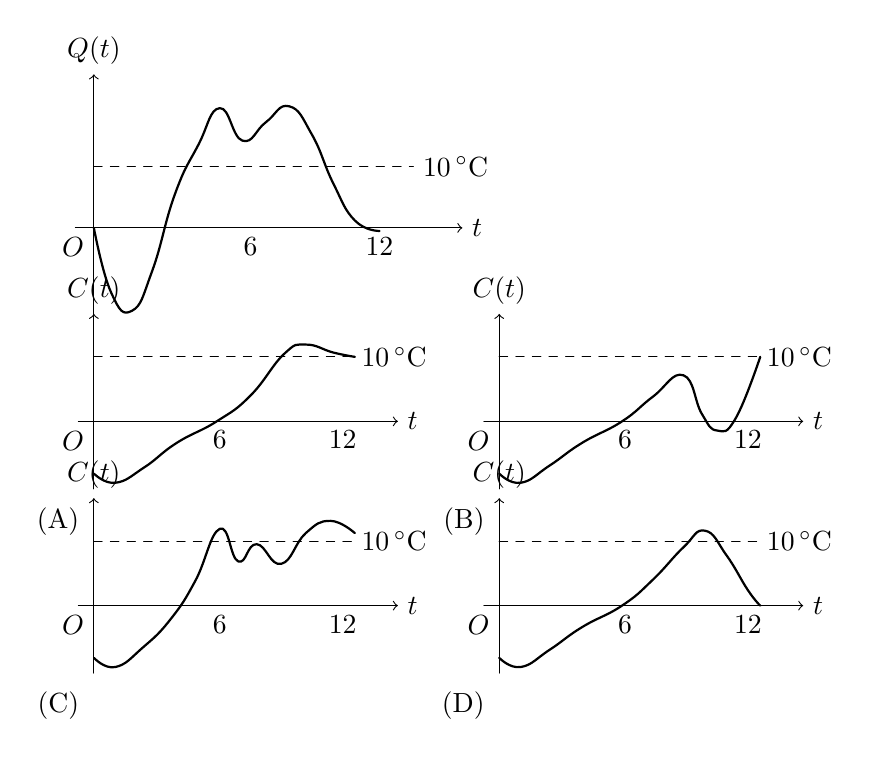
\begin{tikzpicture}[line cap=round,line join=round,scale=0.78]
  % 顶部：气温 Q(t)
  \begin{scope}[shift={(0,5.7)}]
    \draw[->] (-0.3,0)--(6.0,0) node[right] {$t$};
    \draw[->] (0,-1.55)--(0,2.5) node[above] {$Q(t)$};
    \draw[dashed] (0,1.0)--(5.2,1.0) node[right] {$10\,{}^\circ\mathrm C$};
    \draw[thick] plot[smooth,tension=0.82] coordinates
      {(0,0) (0.28,-1.05) (0.62,-1.35) (0.95,-0.7) (1.32,0.55)
       (1.7,1.35) (2.05,1.95) (2.42,1.42) (2.8,1.72) (3.18,1.98)
       (3.55,1.52) (3.9,0.72) (4.25,0.12) (4.65,-0.05)};
    \node[below left] at (0,0) {$O$};
    \node[below] at (2.55,0) {$6$};
    \node[below] at (4.65,0) {$12$};
  \end{scope}

  % 四个选项共用坐标尺度；各曲线只表达原图趋势。
  \foreach \x/\y/\letter in {0/2.55/A,6.6/2.55/B,0/-0.45/C,6.6/-0.45/D}{
    \begin{scope}[shift={(\x,\y)}]
      \draw[->] (-0.25,0)--(4.95,0) node[right] {$t$};
      \draw[->] (0,-1.1)--(0,1.75) node[above] {$C(t)$};
      \draw[dashed] (0,1.05)--(4.2,1.05) node[right] {$10\,{}^\circ\mathrm C$};
      \node[below left] at (0,0) {$O$};
      \node[below] at (2.05,0) {$6$};
      \node[below] at (4.05,0) {$12$};
      \node[below left] at (-0.08,-1.25) {(\letter)};
    \end{scope}
  }
  % (A) 先下降，约在 6 月穿过 0，之后高于 10，最后回到 10。
  \begin{scope}[shift={(0,2.55)}]
    \draw[thick] plot[smooth,tension=0.8] coordinates
      {(0,-0.85) (0.35,-1.0) (0.82,-0.75) (1.35,-0.35)
       (2.0,0) (2.55,0.42) (3.1,1.1) (3.45,1.25)
       (3.9,1.12) (4.25,1.05)};
  \end{scope}
  % (B) 先下降，约在 6 月穿过 0，之后略降至 0 以下再升到 10。
  \begin{scope}[shift={(6.6,2.55)}]
    \draw[thick] plot[smooth,tension=0.8] coordinates
      {(0,-0.85) (0.35,-1.0) (0.82,-0.72) (1.35,-0.35)
       (2.0,0) (2.5,0.4) (3.0,0.75) (3.3,0.12)
       (3.55,-0.15) (3.85,0.05) (4.25,1.05)};
  \end{scope}
  % (C) 先上升越过 10，随后起伏，末端仍在 10 上方。
  \begin{scope}[shift={(0,-0.45)}]
    \draw[thick] plot[smooth,tension=0.8] coordinates
      {(0,-0.85) (0.35,-1.0) (0.8,-0.68) (1.25,-0.22)
       (1.65,0.4) (2.05,1.25) (2.35,0.72) (2.65,1.0)
       (3.05,0.68) (3.45,1.18) (3.85,1.38) (4.25,1.18)};
  \end{scope}
  % (D) 先下降，约在 6 月穿过 0，形成高于 10 的峰后于 12 月回到 0。
  \begin{scope}[shift={(6.6,-0.45)}]
    \draw[thick] plot[smooth,tension=0.8] coordinates
      {(0,-0.85) (0.35,-1.0) (0.82,-0.72) (1.35,-0.35)
       (2.0,0) (2.5,0.42) (3.0,0.95) (3.35,1.22)
       (3.7,0.82) (4.05,0.25) (4.25,0)};
  \end{scope}
\end{tikzpicture}
